%********************************************************************************************
%								COMANDOS ÚTILES PARA LATEX EN ESTE TP							
%
%	\ : espacio simple
%	\\ : nueva línea
%	\par : va a la línea de abajo y deja sangría
%	\vspace{##tamaño en pt##} o \vspace{\baselineskip} en general:
%								 para dejar un espacio vertical
%	\textbf{text} :text en negrita
%	\textit{text} :text en itálica
%
% GRAFICOS CENTRADOS:
%	\begin{center}
%		\includegraphics[width=\textwidth]{./img/##ruta imagen (no hace falta extension)##}
%	\end{center}
%		--> se pueden agregar atributos como scale por si se hace muy grande
%
% TABLAS CENTRADAS:
%	\begin{center}
%	\begin{tabular}{|c|c|}
%	\hline
%	\ \textbf{Programa} & \textbf{Ticks} \\
%	\hline
%		ASM & 675127609 \\
%	\hline
%	\end{tabular}
%	\end{center}
%
% ALGORITMOS (EN VARIOS LENGUAJES):
% \begin{lstlisting}
%	void sumoDiez(int &num)
%	{
%	    num += 10;
%	}
%	
%	int main()
%	{
% 	   int i;
%	    int numeroAProcesar = 20;
%	    for (i = 0; i < 50; i++)
%	    {
%	        sumoDiez(numeroAProcesar);	//Proceso el numero en cada ciclo
%	    } 
%	    return 0;
%	}
%	\end{lstlisting}
%
% para info sobre todo lo que tiene el package detallado:
% http://en.wikibooks.org/wiki/LaTeX/Source\_Code\_Listings
%
%********************************************************************************************

\documentclass[10pt,a4paper]{article}
\usepackage[utf8]{inputenc} % para poder usar tildes en archivos UTF-8
\usepackage[spanish]{babel} % para que comandos como \today den el resultado en castellano
\usepackage{a4wide} % márgenes un poco más anchos que lo usual
\usepackage[conEntregas]{caratula}
\usepackage{amssymb}
\usepackage{amsthm}
\usepackage{fancybox}
\usepackage[usenames,dvipsnames]{color}
\usepackage{hyperref}
\usepackage{listings}
\usepackage{ulem}
\usepackage{color}
\usepackage[table]{xcolor}
\usepackage{amsmath}
\usepackage{float}
\usepackage{pdflscape}
%\usepackage[landscape]{geometry}
\usepackage{pdfpages}


\hypersetup{
    colorlinks,
    citecolor=black,
    filecolor=black,
    linkcolor=black,
    urlcolor=black
}

\lstdefinestyle{customc}{
  belowcaptionskip=1\baselineskip,
  breaklines=true,
  frame=L,
  xleftmargin=\parindent,
  language=C,
  showstringspaces=false,
  basicstyle=\footnotesize\ttfamily,
  keywordstyle=\bfseries\color{green!40!black},
  commentstyle=\itshape\color{purple!40!black},
  identifierstyle=\color{blue},
  stringstyle=\color{orange},
}

\newtheorem{theorem}{Teorema}[section]
\newtheorem{corollary}{Corolario}[theorem]
\newtheorem{lemma}[theorem]{Lema}

\begin{document}

\titulo{Primer parcial}

\fecha{\today}

\materia{Teoria de Juegos}

\integrante{Vileriño, Silvio}{106/12}{svilerino@gmail.com}

\maketitle

\tableofcontents
\newpage

\section{Introducción}
%ya esta el section en informe.tex
%\section{Introducción}
El objetivo de este documento es la resolucion del parcial descripto en la seccion enunciado.

\section{Enunciados}
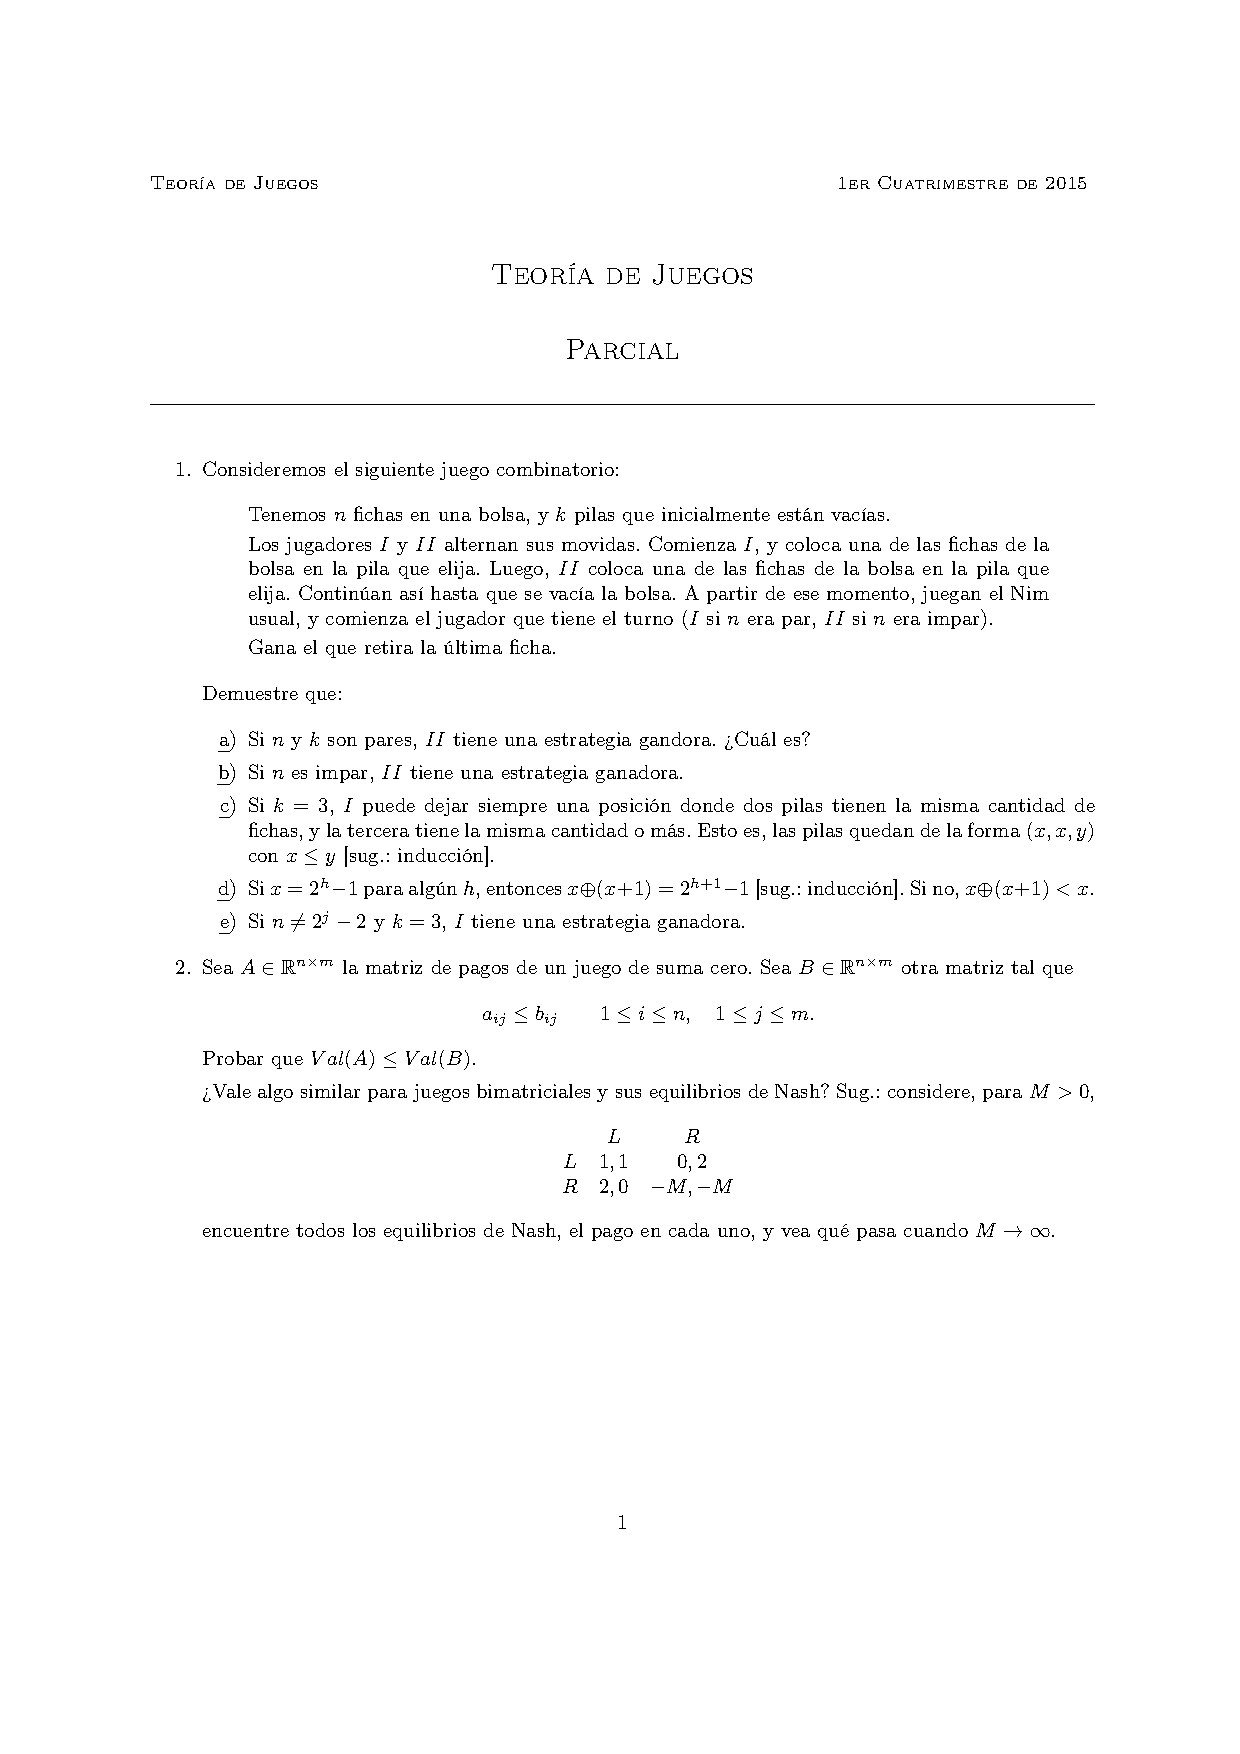
\includepdf[pages=1-2]{include/parcial2015.pdf}

\section{Desarrollo}
\subsection{Combinatorio}
\subsection{Estrategias ganadoras del jugador II}
Para los incisos a) y b) de este ejercicio, definiremos ciertas cosas a continuacion.

\textbf{Nota}: $\bigoplus$ es la suma nim.\\

\begin{theorem}[Teorema de Bouton]
\label{bouton}
	Una posicion $(X_1, \dots, X_n)$ en Nim, es \texttt{P-Position} $\leftrightarrow$ $X_1 \bigoplus ... \bigoplus X_n = 0$ 
\end{theorem}

\begin{theorem}
\label{particion-movidas}
	Las posiciones de un juego se particionan en \texttt{N-Position} y \texttt{P-Position}.
\end{theorem}

\begin{theorem}[Propiedad caracteristica de las posiciones]
	\label{position-characterization}
	Las posiciones de tipo \texttt{N-Position} y \texttt{P-Position} se definen recursivamente como:
	\begin{enumerate}
		\item Todas las posiciones terminales son \texttt{P-Position}.
		\item Desde toda \texttt{N-Position} \textbf{existe al menos una} jugada a una \texttt{P-Position}
		\item Desde toda \texttt{P-Position}, \textbf{todas} las jugadas son hacia \texttt{N-Position}.
	\end{enumerate}
\end{theorem}

\textbf{Idea:} Comenzando en una \texttt{N-Position}, en cada turno del jugador II, este siempre debe moverse a una posicion en la cual el jugador I vuelva a mover a una \texttt{N-Position}.\\

\begin{theorem}[Estrategia ganadora de II]
	\label{estrategia-ganadora}
	Si el jugador II comienza en una \texttt{N-Position}, tiene una estrategia ganadora.	
\end{theorem}
\begin{proof}
	Si el jugador II comienza en una \texttt{N-Position}. Por definicion(\ref{position-characterization}), existe una jugada que me lleva a una \texttt{P-Position}.
	Por definicion de \texttt{P-Position}, el jugador I va a tener que perder el juego porque dicha posicion es terminal o moverse a una \texttt{N-Position}, y nuevamente, el jugador II puede moverse a alguna \texttt{P-Position}. Este proceso se repite y es la estrategia ganadora para el jugador II.\\	
\end{proof}

\begin{corollary}
	\label{estrategia-comienza-I}
	Por definicion de \texttt{P-Position}(\ref{position-characterization}), todas las movidas posibles llevan a una \texttt{N-Position}. Si el jugador I comienza en una \texttt{P-Position}, el jugador II tambien tiene estrategia ganadora desde el momento que I le cede la \texttt{N-Position} al mover o pierde porque es una posicion terminal.
\end{corollary}

\begin{corollary}
	\label{sumanim-posiciones}
	Usando los teoremas \ref{bouton} y \ref{particion-movidas} tenemos que si $(X_1, \dots, X_k)$ es el nim inicial, entonces vale:
	\begin{itemize}
		\item La posicion inicial es una \texttt{P-Position} si $(X_1 \bigoplus \dots \bigoplus X_k) == 0$ 
		\item La posicion inicial es una \texttt{N-Position} si $(X_1 \bigoplus \dots \bigoplus X_k) \neq 0$ 
	\end{itemize}
\end{corollary}

\begin{theorem}[Equivalencia de suma nim a un bitwise exclusive or]
\label{equiv-nim-xor}
	La suma nim es equivalente a aplicar un \textbf{bitwise XOR} a los numeros a y b en base 2. Es decir, podemos definir la suma nim como $a \bigoplus b$ $ = $ $( (a)_2$ $\hat{}$ $(b)_2 )_{10}$.
\end{theorem}
\begin{proof}
	 Se desprende de considerar las tablas de definicion de la suma modulo 2 y la tabla de verdad del xor tomando 0 como falso y 1 como verdadero.
\end{proof}

\subsubsection{Inciso a}
Sabemos que:
\begin{itemize}
	\item El numero n, de fichas en la bolsa, es par
	\item El numero k, de pilas, es par 
\end{itemize}

Dado que n es par, luego de la etapa de colocacion de fichas, comienza jugando el nim el jugador I.\\
Como establecimos en \ref{estrategia-comienza-I} y \ref{sumanim-posiciones}. Si el nim inicial $(X_1, \dots, X_k)$ es tal que $(X_1 \bigoplus \dots \bigoplus X_k) == 0$, el jugador I comenzara en una \texttt{P-Position} y el jugador II tendra la estrategia ganadora mencionada en \ref{estrategia-ganadora}.\\

Solo resta encontrar una manera para que el nim inicial sume cero.\\

\textbf{Idea:} Le balanceo las pilas nim al jugador I de a pares. Luego, en el nim inicial $(X_1, \dots, X_k)$, tengo una cantidad par k de torres tales que:\\
\begin{enumerate}
	\item \textbf{Para cada pila, existe otra con la misma cantidad de elementos:} $\forall $ $ X_j $ $ \in $ $(X_1, \dots, X_k)$ $\exists$ $ X_i $ tal que $ (i \neq j) \land (X_i = X_j) $  
	\item \textbf{Ley de cancelacion de suma nim:} $ (X_i \bigoplus X_j) = 0$  
\end{enumerate}

Por lo tanto, el nim inicial que comienza jugando I es una \texttt{P-Position}. Como queriamos.

\begin{theorem}[Se puede armar un nim inicial que suma cero]
	Bajo estas hipotesis, siempre se puede llegar a un nim balanceado de a pares.
\end{theorem}

\begin{proof}
Por Induccion en cantidad de fichas:\\

Sean:
\begin{itemize}
	\item El numero n, de fichas en la bolsa, natural par no nulo.
	\item El numero k, de pilas, natural par no nulo.
	\item P(n): {Las pilas estan balanceadas(misma cantidad de elementos) de a pares}.
\end{itemize}

Dado que la cantidad de pilas es par, podemos establecer una relacion de apareo entre pares de pilas. Diremos que 2 pilas estan apareadas cuando tienen la misma cantidad de elementos. Concretamente, al final de cada par de turnos tendremos una cantidad par de pares de pilas apareadas.

\begin{itemize}
	\item \textbf{Caso base, n = 2}\\
	Como k es par(y no nulo), entonces $k \geq 2 $. El jugador I coloca una ficha en alguna de las pilas. Luego, existe alguna pila vacia. El jugador II pone una ficha en la pila vacia. Finalmente para toda pila en el nim, o bien esta vacia, o bien es alguna de las 2 pilas con 1 elemento.

	\item \textbf{Caso inductivo, n $\rightarrow$ n+1}
	Vale la hipotesis inductiva. El jugador I coloca una ficha en alguna pila $X_j$. Como las pilas estan balanceadas, existe una pila $X_i$, \texttt{apareada} a $X_j$ tal que si el jugador II coloca una ficha en ella quedan $X_j$ y $X_i$ con la misma cantidad de fichas, balanceadas nuevamente. Como no tocamos ninguna otra pila. Las pilas vuelven a quedar balanceadas.

\end{itemize}
\end{proof}

\subsubsection{Inciso b}
Sabemos que:
\begin{itemize}
	\item El numero n, de fichas en la bolsa, es impar
\end{itemize}

Dado que n es impar, juega primero el jugador II en el nim, queremos que II comience en una \textbf{N-Position}.
Equivalentemente por \ref{sumanim-posiciones}, queremos que la posicion inicial $(X_1, \dots, X_k)$ sume nim \textbf{distinto de cero}, $(X_1 \bigoplus \dots \bigoplus X_k) \neq 0$.

\begin{theorem}
Sea $(X_1, \dots, X_k)$ una posicion en el nim, esta posicion es una \texttt{P-Position} $\leftrightarrow$ $(X_1 \bigoplus \dots \bigoplus X_k) = 0$, usando \ref{equiv-nim-xor} tenemos que:\\

\vspace{0.3cm}

\begin{tabular}{|c|c c|}
			\hline
			& $X_1 	=$ & $	(X_{1,1}, \dots, X_{1,t})_2$ \\\hline
			& $X_2 	=$ & $	(X_{2,1}, \dots, X_{2,t})_2$ \\\hline
$\bigoplus$  & & $ \dots$\\\hline
			& $X_k 	=$ & $	(X_{k,1}, \dots, X_{k,t})_2$ \\\hline 
			& $0$	 & $	(0,   ..., 0)_2$ \\\hline
\end{tabular}
\vspace{0.3cm}

\textbf{Nota:} $t \in \mathbb{N}$ es la cantidad de bits requerida para representar el maximo numero del conjunto ${ X_1, \dots, X_k}$.\\

Esto ocurre unicamente cuando para todo $j$ entre $1$ y $t$ vale que $X_{1,j} + X_{2,j} + \dots + X_{k,j} = 0 $ $ (mod$ $2)$. Es decir, cuando la cantidad de unos en cada una de las columnas es par.\\
\end{theorem}

\begin{proof}
	Es facil ver esto, considerando la asociatividad del XOR en la suma por columna mencionada anteriormente, aplicando la operacion xor de a 2 elementos por columna hasta que finalmente da 0 cuando la cantidad de unos es par, 1 caso contrario.
\end{proof}

\begin{corollary}
	Como nosotros queremos comenzar a jugar el nim en una \textbf{N-Position}, debe existir \textbf{ALGUNA} columna tal que la operacion exclusive or en dicha columna de distinto de cero, es decir, que dicha columna tenga una cantidad \textbf{IMPAR} de unos.
\end{corollary}

\begin{lemma}
	El bit mas a la derecha en la suma nim especificada como operacion exclusive or, indica el bit de paridad del numero $X_j$, es decir. Si dicho bit es 0, el numero $X_j$ es par, caso contrario, el numero $X_j$ es impar.
\end{lemma}

\textbf{Idea:} Conseguir una cantidad impar de torres con cantidad impar de fichas en el armado de las torres.\\

\begin{theorem}[]
	Al ser $n$ impar, el numero de columnas $X_j$ en el nim inicial $(X_1, \dots, X_k)$ tales que $X_j$ es impar,tambien lo sera.
\end{theorem}

\begin{proof}

Sabemos que $n = X_1 + X_2 + \dots + X_n $ y n es impar.

\begin{itemize}
	\item[] Tomando congruencia modulo 2.
	\item[] $n \equiv 1 \equiv X_1 + X_2 + \dots + X_n \equiv $
	\item[] $\sum\limits_{X_k \equiv 1( mod 2 )} X_k$ + $\sum\limits_{X_j \equiv 0( mod 2 )} X_j$
	\item[] Desaparece la sumatoria de los pares por la congruencia.
	\item[] $\equiv \sum\limits_{X_k \equiv 1( mod 2 )} 1$
	\item[] $\equiv t$ $ \equiv $ {Cantidad de pilas impares} 
\end{itemize}

Por lo tanto, por transitividad de la congruencia tenemos que {Cantidad de pilas impares} $\equiv 1$
\end{proof}

Por lo enunciado anteriormente, la suma nim de la posicion nim inicial, sera \textbf{distinta de cero}, que es lo que queriamos ver.
\subsection{Suma Cero}
\subsubsection{Inciso a}
\begin{theorem}[Minimax]
\label{minimax-teo}
	Sea $A \in \mathbb{R}^{n \times m}$ una matriz de pago de un juego de suma cero. Entonces existen $v \in \mathbb{R} $ y p,q vectores de probabilidad. Tales que:
	\begin{itemize}
		\item $v = Val(A) = \displaystyle\max_{p} \{    \displaystyle\min_{q} \{  p^t . A . q \}    \} = \displaystyle\min_{q} \{    \displaystyle\max_{p} \{  p^t . A . q \}    \}$ 
	\end{itemize}
\end{theorem}

\begin{lemma}
\label{lema-fg}
	Sean $A, B \in \mathbb{R}^{n \times m}$ Matrices. Si $a_{ij} \leq b_{ij}$ para $1 \leq i \leq n$   ,  $1 \leq j \leq m$. Entonces $p^t . A . q \leq p^t . B . q$ para todo vector $p \in \mathbb{R}^{n \times 1}$ y $q \in \mathbb{R}^{m \times 1}$ que sean vectores de probabilidad(todos sus elementos suman uno y cada elemento mayor o igual a cero).
\end{lemma}
\begin{proof}
	Si desarrollamos los productos $p^t . A . q$ y $p^t . B . q$ vemos que cada uno es un numero real, y termino a termino se puede aplicar la desigualdad valida por hipotesis. $a_{ij} \leq b_{ij}$.
\end{proof}

\begin{theorem}
	Sea $A \in \mathbb{R}^{n \times m}$ una matriz de pago de un juego de suma cero. Sea $B \in \mathbb{R}^{n \times m}$ otra matriz tal que $a_{ij} \leq b_{ij}$ para $1 \leq i \leq n$   ,  $1 \leq j \leq m$. Entonces $Val(A) \leq Val(B)$.
\end{theorem}
\begin{proof}
	Consideremos las funciones $f:(\Delta_x \times \Delta_y)$ y $g:(\Delta_x \times \Delta_y)$, continuas, donde $\Delta_x$ y $\Delta_y$ son compactos de funciones de probabilidades. Donde f y g estan definidas como:
	\begin{itemize}
		\item $f(p, q) = p^t.A.q$ 
		\item $g(p, q) = p^t.B.q$ 
	\end{itemize}

	Usando el teorema \texttt{Minimax} definido en \ref{minimax-teo}, tenemos que:
	\begin{itemize}
		\item $Val(A) = \displaystyle\min_{q} \{    \displaystyle\max_{p} \{  f(p, q) \}    \}$
		\item $Val(B) = \displaystyle\min_{q} \{    \displaystyle\max_{p} \{  g(p, q) \}    \}$
	\end{itemize}

	Usando el lema \ref{lema-fg} Tenemos que $f(p, q) \leq g(p, q)$   $\forall p \in \Delta_x, q \in \Delta_y$.\\

	%\textbf{Ojo con el orden de como tomar min max y la desigualdad $\leq$}

\begin{enumerate}
	\item Tomando $\displaystyle\max_{p}$ de ambos lados tenemos:\\
	$ \displaystyle\max_{p} f(p, q) \leq  \displaystyle\max_{p} g(p, q)$
	
	\item Tomando $\displaystyle\min_{q}$ de ambos lados tenemos:\\
	$ \displaystyle\min_{q} \displaystyle\max_{p} f(p, q) \leq  \displaystyle\min_{q} \displaystyle\max_{p} g(p, q)$

	\item Por la observacion anterior de \texttt{minimax} tenemos que:\\
	$ Val(A) \leq Val(B)$
\end{enumerate}
Como queriamos ver.



\end{proof}





\subsubsection{Inciso b}

\begin{theorem}
	Vale algo similar para los juegos bimat y sus equilibrios de nash? de ser asi enunciar el teorema y probarlo, sino enunciar que no y dar un contraejemplo en proof.
\end{theorem}
\begin{proof}
	.
\end{proof}

Supongamos un valor $ M > 2$, fijo. Por ejemplo $M = 4$. Luego la matriz de pagos para ambos jugadores queda:

\vspace{0.5cm}
\begin{figure}[H]
  \centering	
$\begin{pmatrix}
	(1,1) & (0, 2) \\
	(2, 0) & (-4, -4)
\end{pmatrix} $
  \caption{Matriz de pagos suponiendo M=4.}
\end{figure}


\vspace{0.5cm}
Dadas las combinaciones de estrategias para ambos jugadores $\{L, R\} \times \{L, R\}$. Analicemos cada una:
\begin{itemize}
	\item \textbf{L, L}: El pago de los jugadores es $(1,1)$, pero vemos que al jugador I, le conviene cambiar a R, pues asi gana 2 y mejora su pago. Analogamente, al jugador II, le conviene cambiar a R, pues asi gana 2, mejorando su pago. Luego esta estrategia no es un equilibrio de nash.   
	\item \textbf{L, R}: El pago de los jugadores es $0, 2$, vemos que en este caso, al jugador I no le conviene cambiar de estrategia porque su pago seria -M, es decir, -4, que es menor que el actual, 2. Analogamente, al jugador II no le conviene cambiar .
	\item \textbf{R, L}: 
	\item \textbf{R, R}: 

\end{itemize}
\subsection{Equilibrios - Nash}
\subsubsection{Inciso a}
Sabemos que:
\begin{itemize}
	\item Rojo es flanders
	\item Azul es homero
	\item $b \in \mathbb{R}_{>0}$ es el beneficio de tener taladro
	\item $c \in \mathbb{R}_{>0}$ es el costo de comprar el taladro
	\item $b > c$ $ \implies $ $ b - c > 0$  
\end{itemize}

\begin{definition}	
Sea $G=(V, E)$ un grafo. 
\begin{itemize}
	\item Sea la funcion $f:V \rightarrow \{v \in V\}$ la funcion que dado un nodo $v \in V$ me devuelve los vecinos.
	\item Sea la funcion $g:V \rightarrow \{Homero, Flanders\}$ que dado un nodo me devuelve la estrategia elegida por el. 
	\item Sea la funcion $h: V \rightarrow \mathbb{R}_{\geq 0}$ que dado un nodo me devuelve la utilidad, definida para las siguientes estrategias como:
	\begin{itemize}
		\item \textbf{Ned flanders:} Jugador v, compra el taladro, su utilidad es $h(v) = b-c > 0$  
		\item \textbf{Homero:} Jugador v, no compra el taladro, y se lo pide a un vecino, su utilidad es
		\begin{itemize}
			\item $h(v) = c$  Si $(\exists w \in f(v)/ g(w) = flanders)$. \texttt{Si tiene algun vecino flanders.}
			\item $h(v) = 0$  \texttt{En caso contrario.}
		\end{itemize}	 
	\end{itemize}
\end{itemize}
\end{definition}

\begin{theorem}
	\label{ida-caracterizacion-nash}
	Un grafo que cumple las siguientes condiciones, corresponde a un equilibrio de nash.
	\begin{itemize}
		\item \textbf{Todos los jugadores flanders tienen todos vecinos homero}. $(\forall v \in V / g(v) = flanders) \implies (\forall w \in f(v), g(w) = homero)$ 

		\item \textbf{Todos los jugadores homero tienen al menos un vecino flanders}. $(\forall v \in V / g(v) = homero) \implies (\exists w \in f(v)/ g(w) = flanders)$ 
	\end{itemize}
\end{theorem}

\begin{proof}
Veamos porque un grafo que cumple estas condiciones representa un equilibrio de nash:
\begin{itemize}
	\item A los jugadores v, que juegan homero, con utilidad $h(v) = b > 0$, no les conviene cambiar a flanders porque de hacerlo, tendrian utilidad $h(v) = b - c < b$. \textbf{Les va mejor pidiendo prestado a su vecino flanders.}
	\item A los jugadores v, que juegan flanders, con utilidad $h(v) = b-c > 0$, no les conviene cambiar a homero porque de hacerlo, tendrian utilidad $h(v) = 0 < b - c$, \textbf{ya que no tienen ningun vecino a quien pedirle el taladro.}
\end{itemize}
\end{proof}

\begin{theorem}
	El grafo de la figura es un equilibrio de nash. 
\end{theorem}
\begin{proof}
Asumiendo que el grafo se extiende fuera del grafico de la misma forma. Lo que se observa es que dicho grafo cumple las condiciones mencionadas en \ref{ida-caracterizacion-nash}.
\end{proof}

\subsubsection{Incisos b y c}

\begin{theorem}
	\label{vuelta-caracterizacion-nash}
	Si un grafo G=(V, E) se corresponde a un equilibrio de nash, entonces valen las condiciones enunciadas en \ref{ida-caracterizacion-nash}.
\end{theorem}
\begin{proof}
	Supongamos que no, es decir que alguna de las siguientes es cierta y sigue siendo un equilibrio:\\
	\begin{enumerate}
		\item \textbf{Existe un jugador flanders que tiene otro vecino flanders}. $(\exists v \in V / g(v) = flanders) \implies (\exists w \in f(v), g(w) = flanders)$ 

		\item \textbf{Existe un jugador homero que tiene todos vecinos homero}. $(\exists v \in V / g(v) = homero) \implies (\forall w \in f(v)/ g(w) = homero)$ 
	\end{enumerate}
	En el primer caso, sea v dicho jugador, le conviene cambiar a homero y mejorar su utilidad de $b-c$ a $b > b-c$. Por lo tanto no es un equilibrio. En el segundo caso, sea dicho jugador w, le conviene cambiar a flanders y mejorar su utilidad de 0 a $b-c >0$. Por lo tanto, tampoco es un equilibrio.
\end{proof}

\begin{corollary}
	\label{sii-nash-caracterizacion}
	Usando \ref{ida-caracterizacion-nash} y \ref{vuelta-caracterizacion-nash}. Podemos decir que un grafo representa un equilibrio de nash $\leftrightarrow$ cumple con las condiciones enunciadas en \ref{ida-caracterizacion-nash}.
\end{corollary}

\begin{definition}
	Dado G=(V, E) un grafo, se define $T \subseteq V$ un conjunto independiente de nodos si y solo si $\forall w,v \in T w \neq v$ la arista $(v, w) \notin E$. Es decir, los nodos de T no tienen links entre ellos.
\end{definition}

\begin{definition}
	Un conjunto independiente maximal T, es aquel conjunto independiente tal que no esta contenido en ningun otro conjunto independiente.
\end{definition}

\begin{definition}
	Dado G=(V, E) un grafo, se define $T \subseteq V$ un conjunto dominante de nodos si $\forall v \in (V \setminus T) $ $\exists w \in T $ tal que $ (v, w) \in E$. En castellano, que todo nodo de $(V \setminus T) $ sea vecino de un elemento de $T$.
\end{definition}

\begin{theorem}
	\label{caracterizacion-conjindepdominante}
	Dado G=(V, E) un grafo que representa un equilibrio de nash, $V = F \cup H$ donde F es el conjunto de los nodos que juegan Flanders y H es el conjunto de nodos que juegan Homero. Usando la caracterizacion de \ref{sii-nash-caracterizacion} y las definiciones anteriores. Notemos que F es un conjunto independiente y dominante. Y podemos definir una particion del conjunto de nodos como $V = F \cup (V \setminus F)$ tal que G sigue representando un equilibrio de nash.
\end{theorem}
\begin{proof}
	Veamos que esta particion del conjunto de nodos $V = S \cup (V \setminus S)$ cumple las 2 condiciones enunciadas en \ref{ida-caracterizacion-nash}.
	\begin{enumerate}
		\item $\forall v \in S $ $(\forall w \in f(v), g(w) = homero) $. De lo contrario habria 2 nodos en $S$ con una arista, absurdo porque $S$ es independiente.
		\item Sea $H = (V \setminus S)$, entonces $(\forall v \in H) \implies (\exists w \in f(v)/ g(w) = flanders)$. De lo contrario habria un nodo en $V = (V \setminus S)$ que no es vecino de un nodo en $V$, absurdo porque $S$ es dominante.
	\end{enumerate}
\end{proof}

\begin{theorem}
	Un conjunto independiente maximal V, es tambien un conjunto dominante.
\end{theorem}
\begin{proof}
	Supongamos que no, luego tenemos un elemento $w \in (V \setminus S)$ tal que $(w, v) \notin E$ para ningun $v \in V$, entonces si considero $T = V \cup \{w\}$ tambien es un conjunto independiente, lo cual es absurdo, porque V era maximal.
\end{proof}

\begin{theorem}
	\label{nash-cjind}
	Dado G=(V, E) un grafo, un algoritmo que me construya un conjunto independiente maximal S, me genera una particion de nodos $V = S \cup (V \setminus S)$ tal que si tomo $V$ como los nodos que juegan flanders y $(V\setminus S)$ como los nodos que juegan homero, tengo un equilibrio de nash. En definitiva, tal algoritmo me genera equilibrios de nash sobre el grafo G.
\end{theorem}
\begin{proof}
	Sale del teorema \ref{caracterizacion-conjindepdominante}.
\end{proof}

\begin{theorem}
	\label{Multiplicidad-cjindmax}
	Sea G = (V, E) un grafo con al menos una arista tiene mas de un conjunto maximal independiente.
\end{theorem}
\begin{proof}
	Consideremos la arista $(v, w)\in E$ que menciona la hipotesis. Ahora consideremos $C_1$ y $C_2$ conjuntos independientes maximales, construidos golosamente a partir de v y w. Debe valer $C_1 \neq C_2$ pues de lo contrario los nodos v, w de la arista estarian en el mismo conjunto independiente, lo cual es absurdo, porque el conjunto es independiente. Luego encontramos mas de un conjunto maximal independiente,como queriamos ver.  

\end{proof}
\begin{theorem}[Existencia de multiples equilibrios de nash]
	Sea G=(V, E) un grafo finito con mas de dos jugadores conectados. Luego existe un equilibrio de nash, y no es unico.
\end{theorem}
\begin{proof}
	Usando los teoremas \ref{nash-cjind} y \ref{Multiplicidad-cjindmax}. Aplicando el algoritmo sobre nodos iniciales v,w tales que $(v,w) \in E$, para que el conjunto independiente computado sea distinto.
\end{proof}

\begin{theorem}[Algoritmo goloso de busqueda de un conjunto maximal]
	Sea G = (V, E), donde V es el conjunto de nodos del grafo, entonces:
	\begin{enumerate}
		\item Sea $I = \emptyset$
		\item Mientras haya nodos en V repetir
		\begin{itemize}
			\item Elegir un nodo $v_i$ de el conjunto $V$
			\item $I = I \cup \{v\} $
			\item $V = V \setminus (\{v\} \cup f(v)) $, donde f(v) son los vecinos del nodo v.
		\end{itemize}
		\item Devolver I.
	\end{enumerate}
	I es un conjunto independiente maximal de G.
\end{theorem}

\subsubsection{Inciso d}

Se pide hallar familias de grafos de n nodos, conexos, tales que:
\begin{enumerate}
	\item \textbf{Una familia de grafos tal que el numero de taladros sea independiente de n.} Vemos que en la familia de nodos $K_n$, o grafos completos, grafos donde estan presentes las aristas entre cada par de nodos, el numero de taladros necesarios para un equilibrio de nash es independiente de n. Mas aun, con un jugador que juegue flanders, y n-1 que jueguen homero. Se cumplen ambas propiedades mencionadas en \ref{ida-caracterizacion-nash}, con las cuales justificamos en el inciso a que es un equilibrio de nash.
	\begin{figure}[H]
	  \centering	
		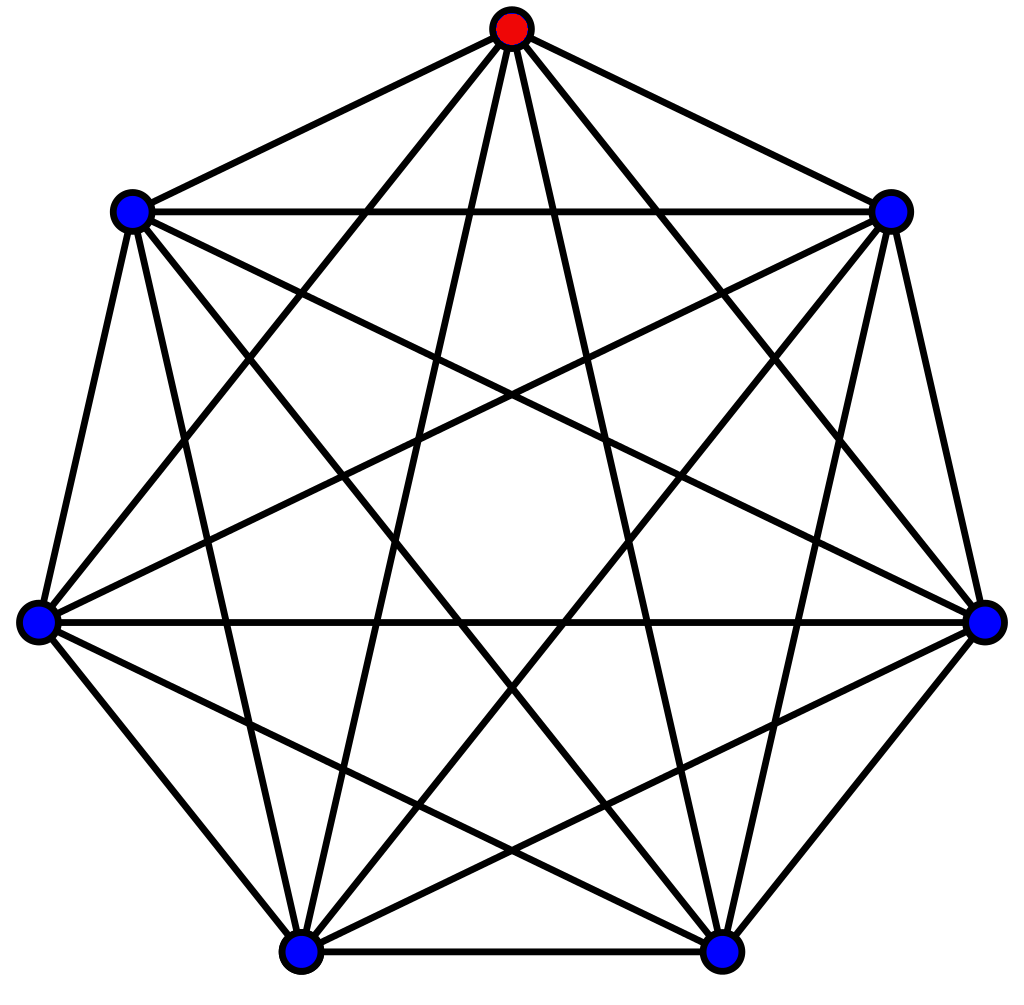
\includegraphics[scale=0.20]{fig/Kn.png}
	  \caption{Grafo del item 3.d.1}
	\end{figure}

	\item \textbf{Una familia de grafos tal que el equilibrio de nash necesita al menos $\frac{n}{2}$ taladros, pero existe una distribucion de taladros tal que 2 sean suficientes para que todos tengan un taladro o tengan un vecino que tenga taladro.} Vemos que para este caso podemos considerar la familia de grafos indicada en las figuras debajo. \ref{3d2} y \ref{3d2b}.
	\begin{figure}[H]
		\label{3d2}
	  \centering	
		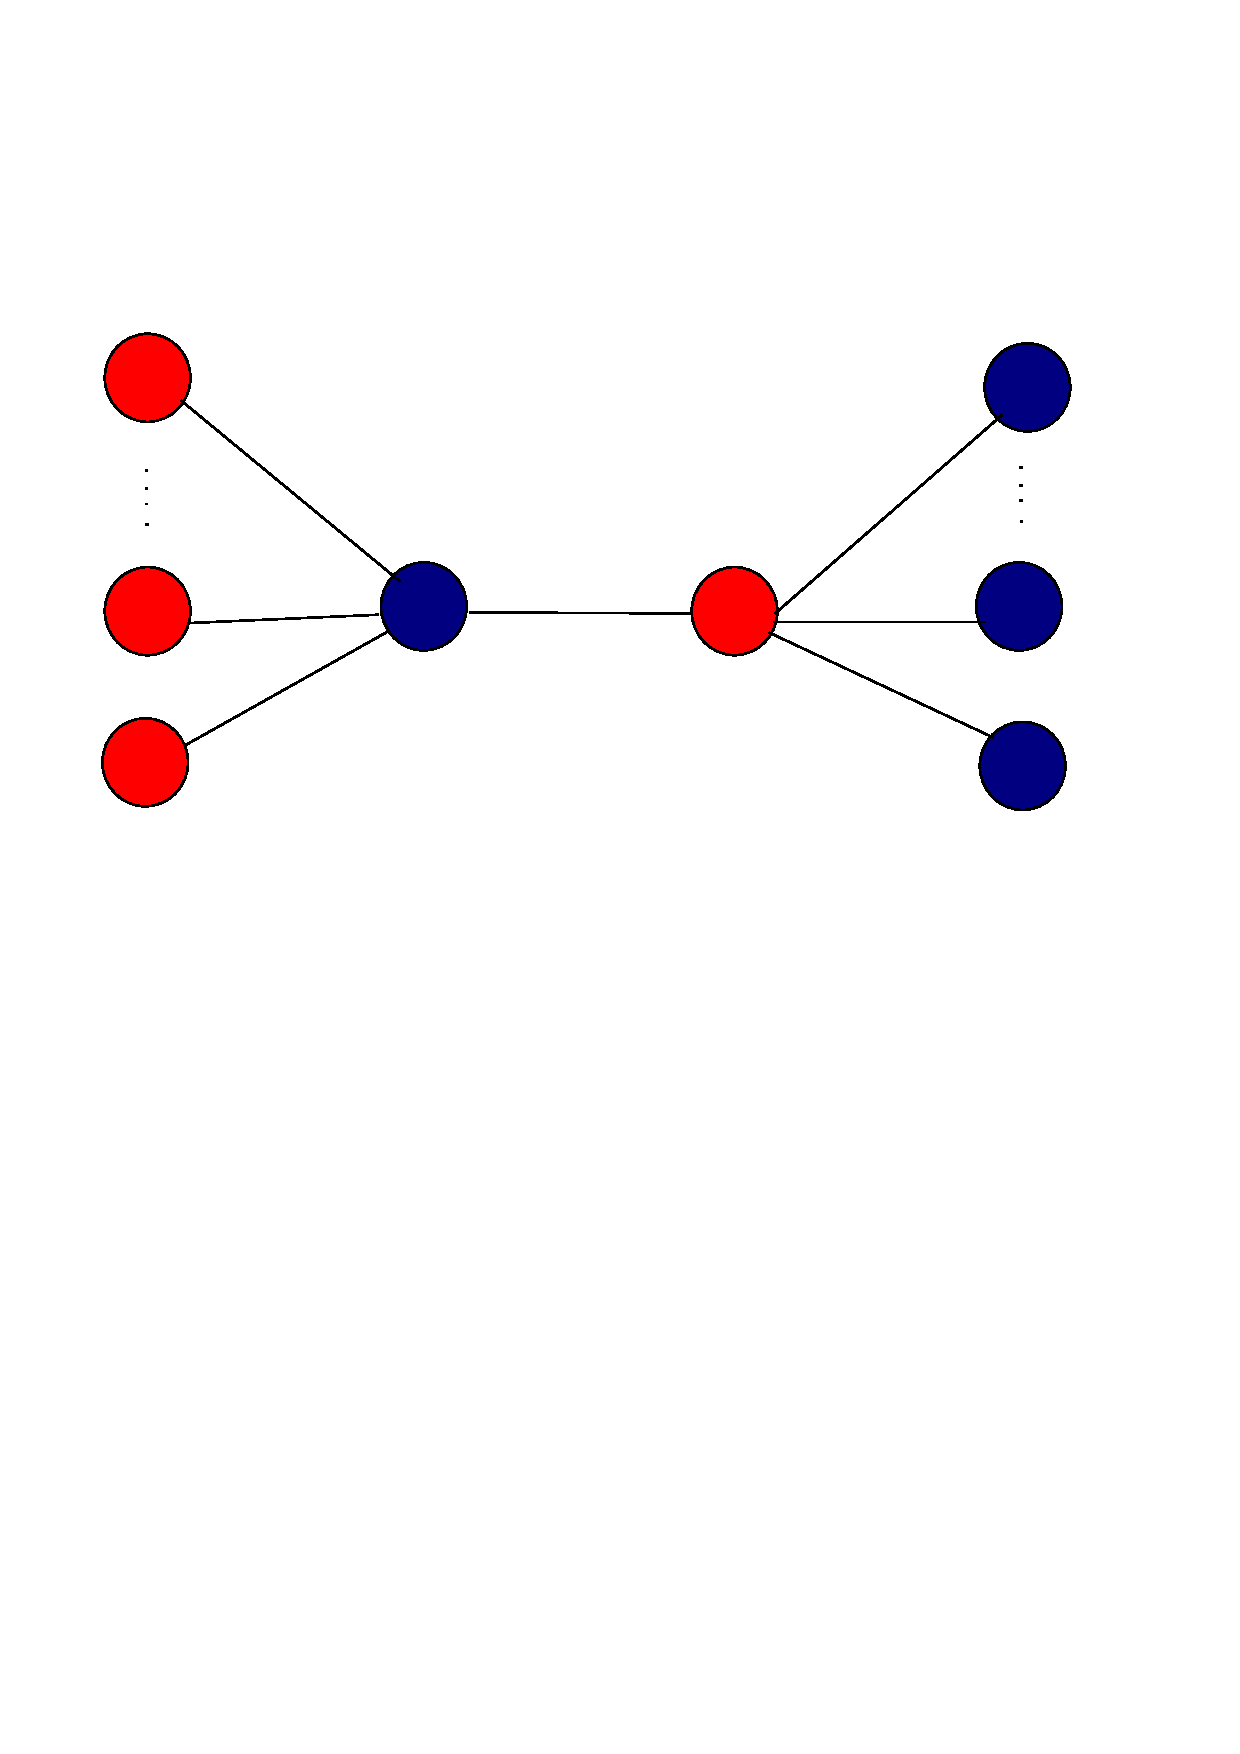
\includegraphics[scale=0.30]{fig/grafo3d2.pdf}
	  \caption{Grafo del item 3.d.2 exhibiendo la condicion de n/2 taladros.}
	\end{figure}

	\begin{figure}[H]
		\label{3d2b}
	  \centering	
		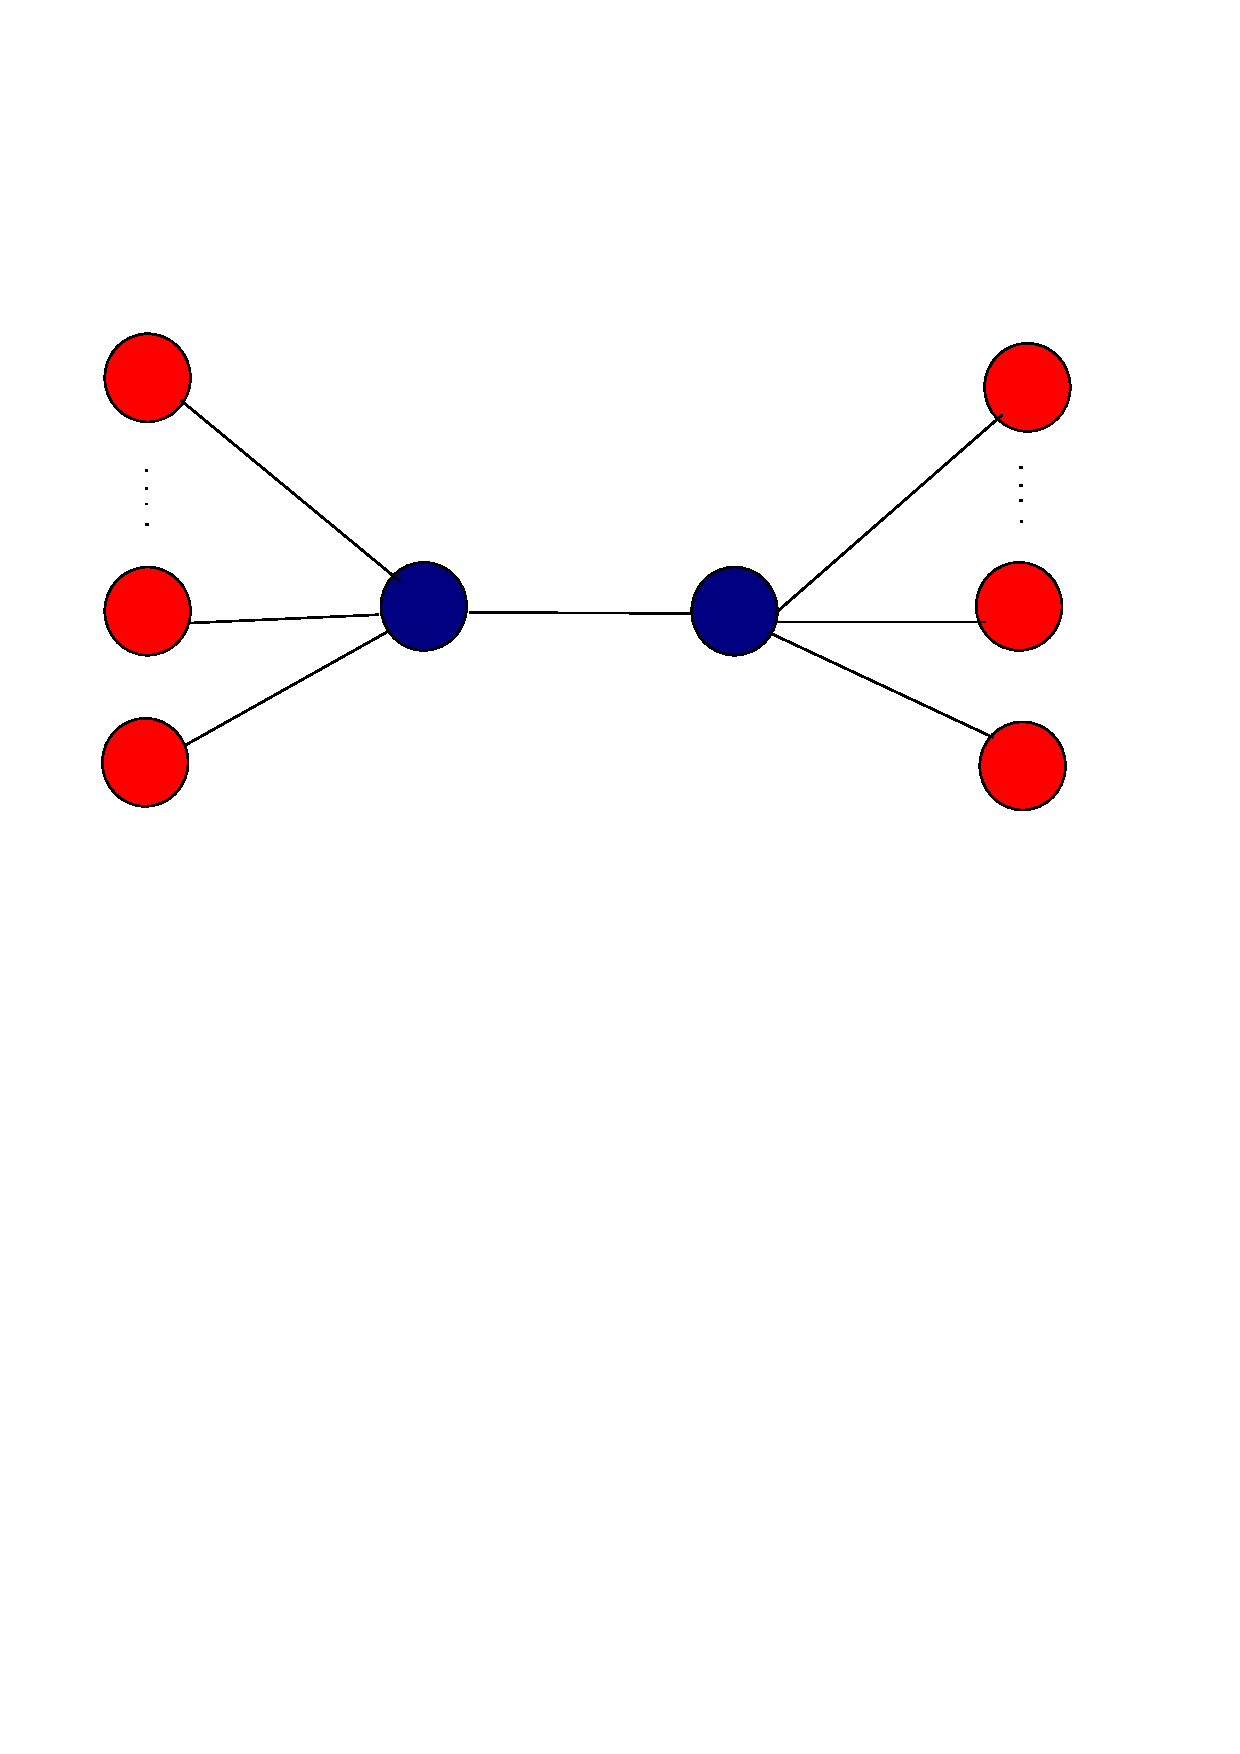
\includegraphics[scale=0.30]{fig/grafo3d2b.pdf}
	  \caption{Grafo del item 3.d.2 exhibiendo la condicion de 2 taladros. \textbf{Estan al reves los colores.}}
	\end{figure}

	\item \textbf{Una familia de grafos tal que todo equilibrio de nash usa aproximadamente una fraccion $\frac{n}k{}, k \in \mathbb{N}$, asumimos que si el grafo es conexo, no es union de grafos disjuntos.(pues hay una arista que los une, entonces no son disjuntos)}. Vemos que es casi una generalizacion del item anterior. Notemos que la fraccion $\frac{n}{k}$ es \textbf{aproximada}. \\
	La idea es tener \texttt{nubes} de $\frac{n}{k}$ nodos sin conexion, cada nube se corresponderia con un grafo ${K_{\frac{n}{k}}}^c$. Luego una arista central, con dos nodos, llamemoslos $v_1$ y $v_2$. El conjunto de aristas del grafo quedaria determinado por las siguientes reglas:
	\begin{enumerate}
		\item $v_1$ y $v_2$ son vecinos.
		\item Para toda nube $n_i$, $i \in\{1,...k-2\}$ , todos sus nodos $n_{i,j}$, estan conectados con $v_1$ y $v_2$ por las aristas $(n_{i,j}, v_1) \in E$ y $(n_{i,j}, v_2) \in E$

		\item La nube $n_{k-1}$ tiene todos sus nodos conectados a $v_1$ por las aristas $(n_{k-1,j}, v_2) \in E$
		\item La nube $n_{k}$ tiene todos sus nodos conectados a $v_2$ por las aristas $(n_{k,j}, v_2) \in E$
	\end{enumerate}
	Las reglas de disposicion de estrategias es como sigue a continuacion:
	\begin{enumerate}
		\item Para toda nube $n_i$, $i \in\{1,...k-1\}$ todos sus nodos juegan homero.
		\item El nodo central $v_1$ juega flanders.
		\item El nodo central $v_2$ juega homero.
		\item La nube $n_k$, tiene todos sus nodos jugando flanders.
	\end{enumerate}
	Puede pensarse una asignacion simetrica cambiando las estrategias de v1 y v2, y las ultimas 2 nubes en la enumeracion.\\
	Es facil ver, dadas estas reglas, que valen las condiciones de \ref{sii-nash-caracterizacion},por lo tanto es un equilibrio de nash. Ademas, veamos que hay asignados $1 + \frac{n}{k}$ taladros.
	\begin{figure}[H]
		\label{3d2b}
	  \centering	
		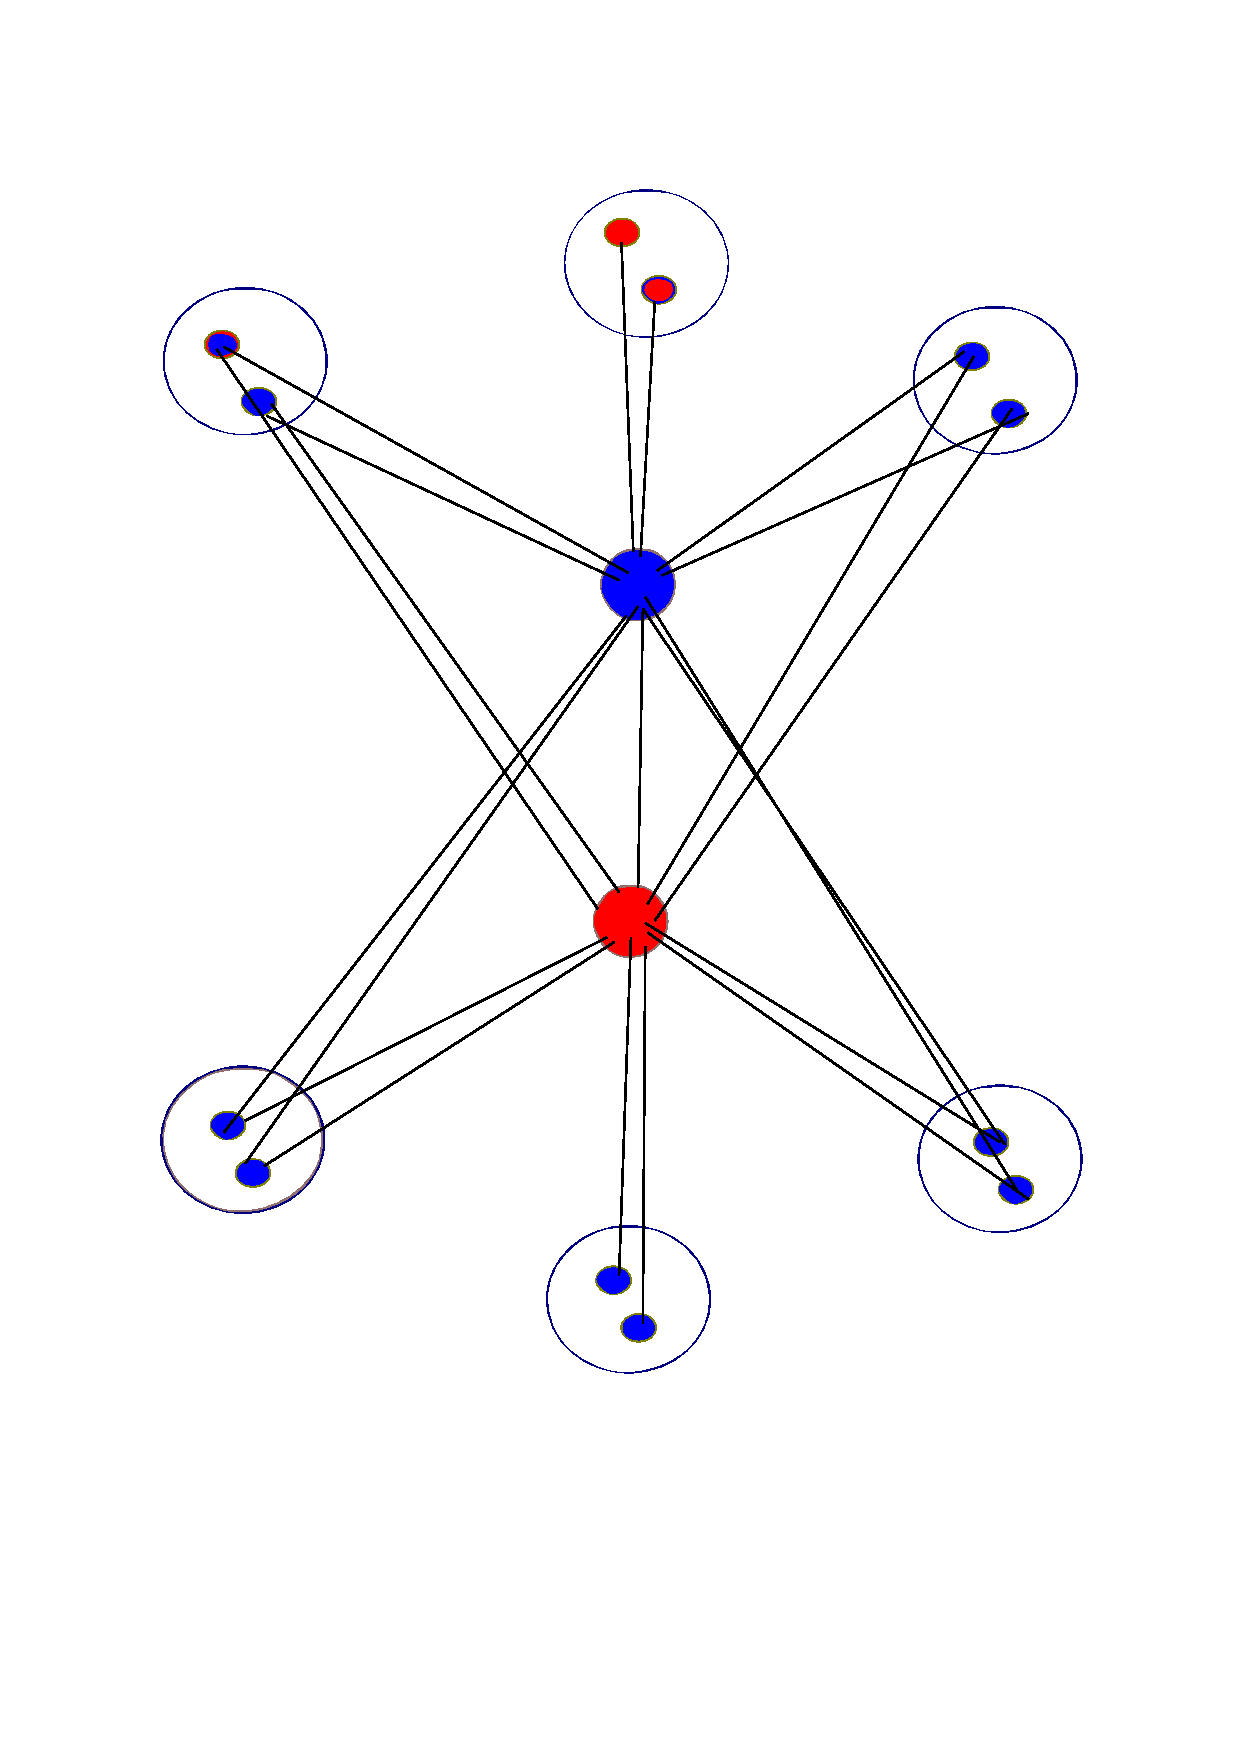
\includegraphics[scale=0.30]{fig/grafo3d3.pdf}
	  \caption{Grafo del item 3.d.3 con n y k fijos.}
	\end{figure}
\end{enumerate}



\end{document}
